\section{Hahn-Banach Theorem \tiny{ (4.2, \cite{Gerald_Teschl})}}
\begin{theorem}[\ifcolor\color{red}\textbf{Hahn-Banach}\color{black}\else Hahn-Banach\fi]
    Assume \(V\) is a real vector space, \(V_0\subset V\) a subspace, \(\phi:V\rightarrow\mathbb{R}\) a convex function (i.e., \(\phi(\lambda x + (1-\lambda)y)\leq \lambda\phi(x) + (1 -\lambda)\phi(y)\)) and 
    \(f:V_0\rightarrow\mathbb{R}\) a linear functional s.t. \(f\leq \phi\) on \(V_0\). Then \(f\) can be extended to a linear functional 
    \(F\) on \(V\) s.t. \(F\leq \phi\).
\end{theorem}
\ifdetailed
\begin{proof}
Assume first that \(V = V_0 + \mathbb{R}x\) for some \(x\in V\backslash V_0\). To define \(F\) we need to specify \(F(x)\). The condition \(F\leq \phi\)
means that we need
\begin{align*}
    F(y\pm tx) \leq \phi(y\pm tx) \ \forall y\in V_0, t\geq 0,
\end{align*}
that is 
\begin{align*}
    \pm t F(x) + f(y) \leq \phi(y\pm tx).
\end{align*}
Dividing by \(t\) this is equivalent to 
\begin{align*}
    \begin{cases} 
        F(x) \leq \frac{\phi(y+tx)-f(y)}{t}, \\
        F(x) \geq \frac{f(y)-\phi(y-tx)}{t}, \\
     \end{cases}
\end{align*}
\(\forall y\in V_0, t\geq0\). To show that there is a number satisfying these inequalities, we need to check that
\begin{align*}
    \sup\limits_{\substack{y\in V_0 \\ t>0}} \frac{f(y)-\phi(y-tx)}{t} \leq \inf\limits_{\substack{y\in V_0 \\ t>0}} \frac{\phi(y+tx)-f(y)}{t}.
\end{align*}
Then as \(F(x)\) we can take any number in the interval \([\sup,\inf]\). In other words, we need to check that
\begin{align*}
    \frac{f(y)-\phi(y-tx)}{t} \leq \frac{\phi(z+sx)-f(z)}{s},
\end{align*}
\(\forall y,z\in V_0, t,s\geq0\). Equivalently, 
\begin{align*}
    sf(y) + tf(z) \leq s\phi(y-tx) + t\phi(z+sx).
\end{align*}
Since \(f\) is a linear functional: \(f(\alpha x) = \alpha f(x), \ \alpha\in K\)(\(=\mathbb{R}\)) and \(x\in V_{0}\), we have
\begin{align*}
    \frac{sf(y) +tf(z)}{s+t} &= f\left(\frac{s}{s+t}y + \frac{t}{s+t}z\right) \\
    &\leq \phi\left(\frac{s}{s+t}y + \frac{t}{s+t}z\right) \\
    &\leq \phi\left(\frac{s}{s+t}(y-tx) + \frac{t}{s+t}(z+sx)\right) \\
    &\leq \frac{s}{s+t}\phi\left(y-tx\right) + \frac{t}{s+t}\phi\left(z+sx\right),
\end{align*}
which is what we need. 

The general case is deduced from this using transitive induction (Zorn's lemma), as follows. Consider the set \(X\) of pairs \((W,F)\), 
where \(w\subset V\) is a subspace, \(F:W\rightarrow \mathbb{R}\) a linear functional, \(V_0\subset W\) and \(F\vert_{v_0} = f\). Define
a partial order on \(X\) by \(F\leq \phi\) on W. 
\begin{align*}
    (W_1, F_1) \leq (W_2, F_2) \text{ iff } W_1\subset W_2\text{ and } F_1=F_2\vert_{W_1}.
\end{align*}
If \(\mathcal{C}\) is a chain in \(X\), then it has an upper bound \((W,F)\) defined by
\begin{align*}
    W = \bigcup\limits_{(Y,\rho)\in\mathcal{C}} Y, F(y) = \rho(y) \text{ if } y\in Y, (Y,\rho) \in\mathcal{C}.
\end{align*}
Hence, \(X\) has a maximal element \((W,F)\) by Zorn's lemma. If \(W\neq V\), then we can take \(x\in V\backslash W\) and extend \(F\) to
\(W+\mathbb{R}x\) preserving the inequality \(F\leq e\). This contradicts maximality of \(W,F\) in \(X\). Hence, \(W=V\).
\end{proof}
\fi 
\begin{theorem}[\ifcolor\color{red}\textbf{Hahn-Banach}\color{black}\else Hahn-Banach\fi]
    Assume \(V\) is a real or complex vector space, \(p\) a seminorm on \(V\), \(V_0\subset V\), and \(f\) a linear functional on \(V_0\) s.t.
    \begin{align*}
        |f(x)|\leq p(x) \ \forall x\in V_0.
    \end{align*}
    Then \(f\) can be extended to a linear functional \(F\) on \(V\) s.t. \(|F(x)|\leq p(x) \ \forall x\in V\).
\end{theorem}
\begin{corollary}
    Assume \(V\) is a normed real or complex vector space, \(V_0\subset V\) is a subspace and \(f\in V_{0}^{*}\). Then there is a \(F\in V^*\) s.t. 
    \begin{align*}
        F\vert_{V_0} = f \text{ and } ||F|| = ||f||.
    \end{align*}
\end{corollary}
\ifdetailed
\begin{proof}
    We apply the previous theorem to \(p(x)=||f||\cdot ||x||\).
\end{proof}
\fi 
% \begin{theorem}[\colortheorem{Hahn-Banach (dense subsets)}]
%     Assume \(\mathcal{H}_0\) is a dense subset of a normed vector space \(\mathcal{H}\) and that \(T:\mathcal{H}_0\rightarrow Y\) is a bounded linear operator (where \(Y\) is a complete, normed vector space), then there is a unique extension of \(T\) to \(T':\mathcal{H}\rightarrow Y\).
% \end{theorem}
\begin{corollary}
    Assume \(V\) is a normed space and \(x\in V, x\neq0\). Then there is a \(F\in V^*\) s.t. \(||F||=1\) and \(F(x) = ||x||\).
\end{corollary}
\ifdetailed
\begin{proof}
We apply the previous corollary to \(V_0 = \mathbb{K}x\) (\(\mathbb{K}=\mathbb{R},\mathbb{C}\)) and \(f:V_0\rightarrow \mathbb{K}\) defined by \(f(cx) = c||x||\).
\end{proof}
\fi
Such an \(F\) is called a \colordefinition{supporting functional at x}. 
\begin{figure}[H]
    \centering
    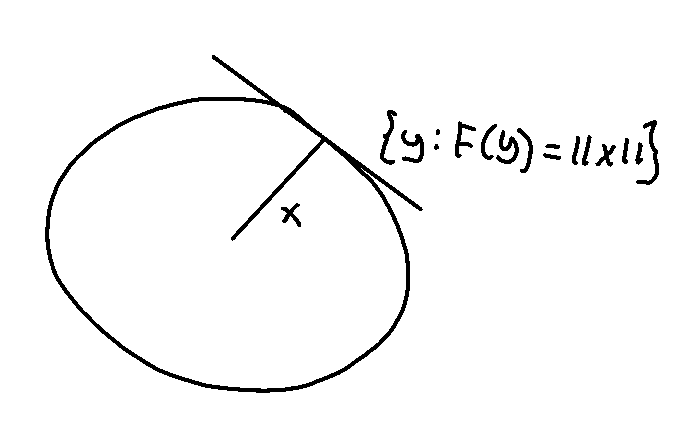
\includegraphics[scale=0.4]{../Figs/hanah_banach1.png}
    \caption{Tangent space?}
\end{figure}
If \(V\) is a normed vector space, then every \(x\in X\) defines a bounded linear functional on \(V^*\) by 
\begin{align*}
    V^*\ni f\mapsto f(x).
\end{align*}
As \(|f(x)|\leq ||f||\cdot ||x||\), this functional has norm \(\leq ||x||\). By using a supporting functional at \(x\), we actually see that
we get norm \(||x||\). Thus, we have an isometric embedding \(V\subset V^{**}\eqdef (V^*)^*\). We can therefor see view \(V\) as a subspace
of \(V^{**}\).
\begin{definition}
    A normed space \(V\) is called reflexive if \(V^{**}=V\).
\end{definition}
\begin{remark}
    This is stronger than requiring \(V\backsimeq V^{**}\). And:
    \begin{enumerate}[label=(\roman*)]
    \item Every finite dimensional normed vector space \(V\) is reflexive for dimension reasons: \(\dim V^{**} = \dim V^*=\dim V\).
    \item Every Hilbert space \(\mathcal{H}\) is reflexive. Indeed, \(\mathcal{H}^*=\overline{\mathcal{H}}\). By Riesz' theorem every bounded linear 
    functional \(f\) on \(\overline{\mathcal{H}}\) has the form
    \begin{align*}
        f(\overline{x}) = (\overline{x}, \overline{y}) = (y,x),
    \end{align*}
    for some \(y\in\mathcal{H}\), which exactly means that \(f=y\) in \(\mathcal{H}^{**}\).
    \end{enumerate}
\end{remark}
As we will see later, the spaces \(\mathcal{L}^{p}(X,d\mu)\), with \(\mu\) \(\sigma\)-finite and \(1<p<\infty\), are reflexive. The spaces
\(\mathcal{L}^{1}(X, d\mu)\) and \(\mathcal{L}^{\infty}(X,\mu)\) are usually not reflexive.
